%figure 1
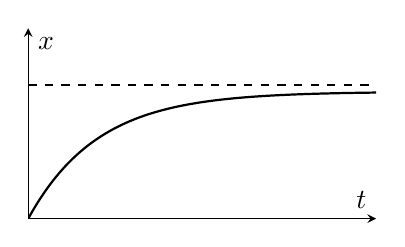
\begin{tikzpicture}
    \begin{axis}[
        axis lines=middle, 
        xlabel={$t$}, 
        ylabel={$x$},
        xmin=0, xmax=5, ymin=0, ymax=1.5,
        xtick=\empty, ytick=\empty,
        domain=0:5,
        samples=100,
        width=6cm,
        height=4cm,
    ]
    \addplot[smooth, thick] {1 - exp(-x)}; 
    \addplot[dashed, thick] coordinates {(0,1.05) (5,1.05)}; 
    \end{axis}
\end{tikzpicture}
%figure 2
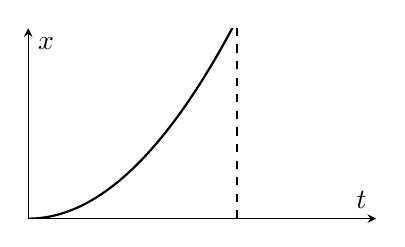
\begin{tikzpicture}
    \begin{axis}[
        axis lines=middle, 
        xlabel={$t$}, 
        ylabel={$x$},
        xmin=0, xmax=5, ymin=0, ymax=8.6, 
        xtick=\empty, ytick=\empty,
        domain=0:5,
        samples=100,
        width=6cm,
        height=4cm,
    ]
    \addplot[smooth, thick] {x^2}; 
    \addplot[dashed, thick] coordinates {(3,0) (3,9)}; 
    \end{axis}
\end{tikzpicture}
%figure 3
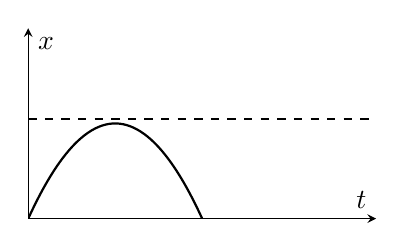
\begin{tikzpicture}
    \begin{axis}[
        axis lines=middle, 
        xlabel={$t$}, 
        ylabel={$x$},
        xmin=0, xmax=4, ymin=0, ymax=2,
        xtick=\empty, ytick=\empty,
        domain=0:4,
        samples=100,
        width=6cm,
        height=4cm,
    ]
    % Function: y = x(2 - x)
    \addplot[smooth, thick] {x * (2 - x)};
    
    % Calculate the maximum y-coordinate
    \pgfmathsetmacro{\maxY}{1}  % Maximum occurs at x=1
    \pgfmathsetmacro{\offset}{0.05}  % Small offset to position dashed line above the maxY
    
    % Horizontal dashed line just above the maximum point
    \addplot[dashed, thick] coordinates {(0, \maxY + \offset) (4, \maxY + \offset)}; 

    \end{axis}
\end{tikzpicture}
%figure 4
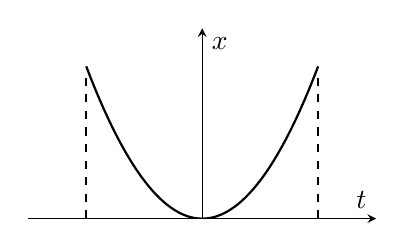
\begin{tikzpicture}
    \begin{axis}[
        axis lines=middle, 
        xlabel={$t$}, 
        ylabel={$x$},
        xmin=-3, xmax=3, ymin=0, ymax=5,
        xtick=\empty, ytick=\empty,
        domain=-2:2, 
        samples=100,
        width=6cm,
        height=4cm
    ]
    \addplot[smooth, thick] {x^2}; 
    \addplot[dashed, thick] coordinates {(-2,0) (-2,3.7)};
    \addplot[dashed, thick] coordinates {(2,0) (2,3.7)};
    \end{axis}
\end{tikzpicture}
